\chapter{微软Edx语音识别笔记}
本章笔记主要是对微软Edx的课程\href{https://courses.edx.org/courses/course-v1:Microsoft+DEV287x+1T2019a/course/}{Speech Recognition System}的记录,首版主要是翻译,再加上自己翻阅其他资料综合起来的一些思考和总结。代码见\href{https://github.com/MicrosoftLearning/Speech-Recognition}{Speech-Recognition}

%------------------------------------------------------------------------------
%                                Fundamentals
%------------------------------------------------------------------------------
\section{Background and Fundamentals}
\subsection{Phonetics} % (fold)
\label{ssub:phonetics}
Phonetics(语音学)是Linguistics(语言学)的一个分支,其研究的是人类语音发出的声音(sound)。语音学围绕着声音的产生(通过人类的发音器官)、声音的声学特性和感知。语音学有三个基本的分支,这三个分支都与ASR有关系。
\begin{enumerate}
	\item Articulatory Phonetics(发音语音学):通过发音器官、不同说话人而产生的声音;
	\item Acoustic Phonetics(声学语音学):声音从说话人到听者的传输;
	\item Auditory Phonetics(听觉语音学):听者对于声音的接收和感知。
\end{enumerate}

声音的最小单元我们成为\textcolor{red}{Phoneme},即音素。序列中的词(Words)是由一个或多个音素组成的。一个音素的声学实现称为\textcolor{red}{Phone}。图\ref{fig:exam-phonemes}展示了美式英语的音素和一般实现办法。
\begin{figure}[htbp]
  \centering
  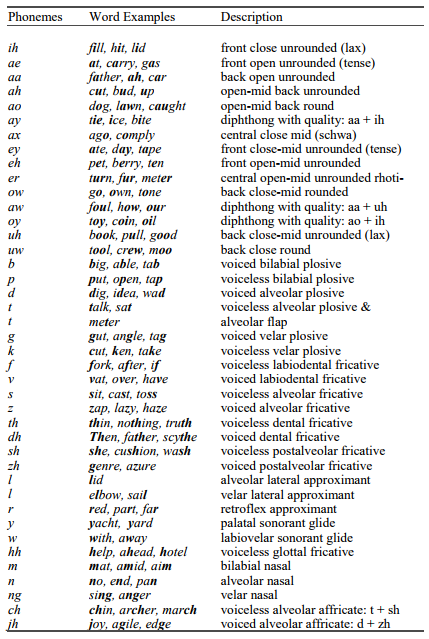
\includegraphics[width=0.35\textwidth]{phonemes}
  \caption{美式英语的音素和一般实现办法 \label{fig:exam-phonemes}}
\end{figure}

一般我们将音素分为两类:元音(Vowel)和辅音(Consonants)。
\begin{enumerate}
	\item Vowels:元音有两个特点,一是元音都是发声的声音(voiced sound),这意味着从声带(vocal chords)到口腔(mouth cavity)的气流是由声带的某种基频的震动(或者音高)产生的。二是舌头在生产过程中不会以任何方式形成气流收缩。每个元音发声的时候舌头、嘴唇和下巴的造型都不一样。这些不同的方式形成了不同的共振态,我们称之为共振峰。这些共振峰的共振态频率形成了不同的元音。
	\item Consonants:辅音是通过在口腔中或者空气中很明显的气流收缩形成的。有些辅音和元音一样是发声的,有些是不发声的。不发声的音素不会激活声带,因此也不存在基频或者音高。一些辅音音调成对出现,只有在有声或无声的情况下才有所不同,但在其他方面是相同的。比如说/b/和/p/这两个音素的发音方式是相同的,因为你的嘴唇、下巴还有舌头的姿势是一样的。但是/b/是发声的,/p/是不发声的。
\end{enumerate}

音素的另外一个重要特性是\textcolor{red}{其根据不同的上下文音素发音是会改变的}。我们称之为Phonetic Context。之所以会这样,是因为协同发音(coarticulation)。这些声音连续起来发音会改变其原有的特征。由协同发音产生的音素我们称为音素变体(allophones)。

所有当前的这些语音识别系统都使用了音素的语境相关的特性来建立处于不同phonetic context的音素模型。
% subsubsection phonetics (end)

\subsection{Words and Syntax} % (fold)
\label{sub:words_and_syntax}
Syllable 是一串声音,是个序列,由一个核心的音素,可能有初始音素和终止音素,这个核心音素一般是个元音或者一个音节辅音(syllablic consonant),是能够唱出来或者吼出来的声音。

举个例子,英文单词 "bottle" 包含两个 syllable 。第一个 syllable 有三个 phone ,在 Arpabet 音素描述代码里,是 "b aa t" 。这个 "aa" 就是核心音素,"b" 是发声的初始音素,"t" 是不发音的终止音素;第二个 syllable 是只包含一个 syllablic cosonant "l"。

一个 syllable 也可以组成一个词,其本身就是一个单独的音素,比如说,"Eye","uh",或者"eau"(医:水)。

语音识别里面,syllable 很少会考虑作为声学模型的建模单元,而词一般是变成音素来建模。

Syntax(句法规则)描述了给定词和定义了语法的规则下,句子的形成。而 Semantics(语义学)一般指代的是句子中的词或者短语是如何形成句意的。Syntax 和 Semantics 是 NLP 的重要组成部分,但是在语音识别里面,不起主要作用。
% subsection words_and_syntax (end)

\subsection{Measuring Performance} % (fold)
\label{sub:measuring_performance}
在语音识别系统的搭建和实验中,如何来衡量一个系统的好坏呢?由于语音识别是一个序列任务,跟图像当中的分类不一样,因此我们在衡量系统的性能时需要考虑到整个序列。

语音识别准确率衡量最常用的一个指标是词错误率(word error rate,WER)。一般识别出来的结果可能会产生三种错误:替换(substitution)、删除(delete)和插入(insert)。替换指的是一个词被识别成了另外一个词;删除指的是原本有词,但是没有识别出来;插入指的是原本没有词,多识别出来了词。WER 的计算方式如公式\ref{eqn:wer}。
\begin{align}
\label{eqn:wer}
  WER = \frac{N_{sub}+N_{ins}+N_{del}}{N_{ref}}
\end{align}
其中$N_{sub}$、$N_{ins}$和$N_{del}$分别是替换、插入和删除的数量,而$N_{ref}$是参考文本描述中词的个数。

WER的计算用的是通过计算实际输出描述和参考文本描述之间的\href{https://en.wikipedia.org/wiki/Edit_distance}{字符串编辑距离}得到的。编辑距离的实现通过动态规划算法。因为长文本的编辑距离可能不可靠,所以我们通过逐句的计算累积的错误,这些错误最终整合到一起来计算测试集的WER。

表\ref{tab:wer}呈现了实际输出和参考文献之间的不同,以及对应的三种错误。
\begin{lstlisting}[language = python, numbers=left, 
         numberstyle=\tiny,keywordstyle=\color{blue!70},
         commentstyle=\color{red!50!green!50!blue!50},frame=shadowbox,
         rulesepcolor=\color{red!20!green!20!blue!20},basicstyle=\ttfamily]
Ref: however a little later we had a comfortable chat
Hyp: how never a little later he had comfortable chat
\end{lstlisting}
\begin{table}[h]
 \centering
 \caption{WER计算公式中的三种错误实例演示}
   \begin{tabular*}{1\textwidth}{@{\extracolsep{\fill}}ccc}
   \toprule
    {\bf Reference} & {\bf Hypothesis} & {\bf Error} \\
   \midrule
   however      &        how  & Substitution \\ \hline
                &      never  &  Insertion   \\ \hline
         a      &          a  &              \\ \hline
    little      &     little  &              \\ \hline
    later       &      later  &              \\ \hline
    we          &         he  & Substitution  \\ \hline
    had         &        had  &              \\ \hline
    a           &             &   Deletion   \\ \hline
	comfortable   & comfortable &              \\ \hline
      chat      &       chat  &              \\
   \bottomrule
   \end{tabular*}%
 \label{tab:wer}%
\end{table}%

在某些情况中,这三种错误的成本不对等,那么计算编辑距离的时候可以作相应的调整。

句错误率(Sentence Error Rate,SER)是另外一种衡量系统的标准,其计算方式是整句没有出现任何错误。SER 仅仅作为一个指标,来看下错误的句子占全部句子的比例。

% subsection measuring_performance (end)

\subsection{Significance Testing} % (fold)
\label{sub:significance_testing}
统计显著性检验(statistical significance testing)涉及测量两个实验(或算法)之间的差异在多大程度上归因于两个算法中的实际差异,或者仅仅是数据,实验设置或其他因素中的结果固有变异性。统计显著性是所有分类任务的基石,只是统计显著性检验的方法取决于任务的特性。大多数方法的核心是假设检验的概念中存在一个无效假设。问题在于你有多大的confidence能够说无效假设会被拒绝。

对于语音识别来说,比较两个实验或者算法最常用的方法是 Matched Pairs Sentence-Segment Word Error(MAPSSWE)检验,简称为 Matched Pairs Test\upcite{asr-sign}。

在这个方法中,测试集被分为几份,假设这些子测试集中任意一个的错误都与其他子测试集统计独立。这个假设和语音识别的实验很贴合,因为测试数据都是一句一句的经由识别器输出结果。给定了每一个句子的WER,就很容易构建一个matched pairs\upcite{Pallet1990Tools}。
% subsection significance_testing (end)

\subsection{Other Consideration} % (fold)
\label{sub:other_consideration}
除去准确率,对识别系统性能的影响还可能包括计算需求,处理速度或者延迟什么的。解码速度一般用实时因子(real-time factor,RTF)来衡量。RTF为1.0指的是系统处理10s的数据需要花10s的时间。

RTF高于1.0意味着系统要花更多的时间来解码,对于某些应用,也许是可以接受的,比如希望获得一个会议或者讲座的转写,相对于快速的得到转写结果,准确率可能更重要一些,因此多花一些时间也是可以接受的。

当RTF低于1.0,系统会在当前数据达到前就处理好了之前的数据。当不止一个系统在同一个机器上运行的时候,这个就比较有用了。在这种情况下,我们可以用多线程来并行处理多路音频流。此外RTF低于1.0意味着系统能够满足在线实时解码的音频流应用。比如说,当我们在处理一个手机上远程音频需求的时候,网络阻塞可能会使得服务器接收音频产生间隙和延迟。如果语音识别器能够以比实时更快的速度来处理,那么它就可以在数据达到之后迅速跟进,追上最新的音频进度,以速度来掩盖网络的延迟。

一般来说,语音识别系统能够在准确率和速度之间调整,但是这种调整也是有限的,不可能无限好或者无限快。对于一个给定的模型和测试集,speed-accuracy图有一条不可被突破的渐近线(asymptote),即便给予无限的算力。所以准确率是有个极限的,这个时候的错误率可以认为就是模型带来的错误。一旦根据模型搜索找到了最好的结果,进一步的处理也不会带来准确率上的提升。
% subsection other_consideration (end)

\subsection{The Fundamental Equation} % (fold)
\label{sub:the_fundamental_equation}
语音识别可以看作一个优化任务。特别地,给定一个观测序列$O=\{O_{1},...,O_{N}\}$,我们找寻的是最有可能的词序列$W=\{W_1,...,W_M\}$,也就是说我们要找到最大化后验概率$P(W|O)$的词序列,如公式\ref{eqn:fundamental-equation}。
\begin{align}
\label{eqn:fundamental-equation}
  \hat{W} = \arg\mathop{\max}_{W} P(W|O)
\end{align}
利用贝叶斯规则,我们得到公式\ref{eqn:fun-bayes}。
\begin{align}
\label{eqn:fun-bayes}
  P(W|O) = \frac{P(W)P(O|W)}{P(O)}
\end{align}

因为词序列并不依赖于观测序列的边缘概率分布$P(O)$,我们可以忽略这个部分,综合上述两个公式,我们得到公式\ref{eqn:fun-final}。
\begin{align}
\label{eqn:fun-final}
  \hat{W} = \arg\mathop{\max}_{W} P(W)P(O|W)
\end{align}

这就是语音识别的基本公式。语音识别问题就可以看作是在这个联合模型上的搜索。

公式中的$P(O|W)$叫做\textcolor{red}{声学模型(acoustic model)}。这个模型描述了在给定词序列$W$的条件下,声学观测$O$的分布。声学模型表征的是词序列是如何转换成声学实现的,进而转换成ASR系统的声学观测的。

公式中的$P(W)$叫做\textcolor{red}{语言模型(language model)},其只取决于词序列$W$。语言模型给每一个可能的词序列一个概率值。它是由日常使用的一些词序列训练成的。一个训练好的英语语言模型会给"I like turtles"高的概率值,给"Turtles sing table"低的概率值。语言模型促使着词序列的搜索沿着训练数据中的模式开展。语言模型也可以在一些纯文本的应用中见到,比如浏览器的自动补全等。

由于诸多原因,构建一个语音识别系统比这个简单地公式所能呈现的要复杂的多得多。
% subsection the_fundamental_equation (end)
\subsection{Lab 1: Create a speech recognition scoring program} % (fold)
\label{sub:lab-1}
本模块有一个实验作业,标题为"Create a speech recognition scoring program"。

{\bf Required files:}
\begin{itemize}
	\item \textcolor{blue}{wer.py}
	\item \textcolor{blue}{M1\_score.py}
\end{itemize}}

{\bf Instructions:}

In this lab, you will write a program in Python to compute the word error rate (WER) and sentence error rate (SER) for a test corpus. A set of hypothesized transcriptions from a speech recognition system and a set of reference transcriptions with the correct word sequences will be provided for you.

This lab assumes the transcriptions are in a format called the "trn" format, created by NIST. The format is as follows. The transcription is output on a single line followed by a single space and then the root name of the file, without any extension, in parentheses. For example, the audio file "tongue\_twister.wav" would have a transcription

sally sells seashells by the seashore (tongue\_twister)

Notice that the transcription does not have any punctuation or capitalization, nor any other formatting (e.g. converting "doctor" to "dr.", or "eight" to "8"). This formatting is called "Inverse Text Normalization" and is not part of this course.

The python code \textcolor{blue}{M1\_Score.py} and \textcolor{blue}{wer.py} contain the scaffolding for the first lab. A main function parses the command line arguments and string\_edit\_distance() computes the string edit distance between two strings.

Add code to read the trn files for the hypothesis and reference transcriptions, to compute the edit distance on each, and to aggregate the error counts. Your code should report:
\begin{itemize}
	\item Total number of reference sentences in the test set
	\item Number of sentences with an error
	\item Sentence error rate as a percentage
	\item Total number of reference words
	\item Total number of word errors
	\item Total number of word substitutions, insertions, and deletions
	\item The percentage of total errors (WER) and percentage of substitutions, insertions, and deletions
\end{itemize}

The specific format for outputting this information is up to you. Note that you should not assume that the order of sentences in the reference and hypothesis trn files is consistent. You should use the utterance name as the key between the two transcriptions.

When you believe your code is working, use it to process hyp.trn and ref.trn in the misc directory, and compare your answers to the solution.
% subsection lab (end)

%------------------------------------------------------------------------------
%                                Speech Signal Processing
%------------------------------------------------------------------------------
\section{Speech Signal Processing}
\subsection{Introduction} % (fold)
\label{sub:introduction}
通过空气传播的音频波形通过麦克风的捕捉,将这些压力波转换成可捕捉的电信号活动。对这些电信号活动进行采样,这样就得到了一系列采样波形,我们用这些波形来描述信号。音乐信号一般采样率为 44100 Hz,即一秒钟会有44100个采样点。根据奈奎斯特定理(Nyquist theorem),只有频率低于22050 Hz的音频才可以被捕捉到。如果信号的高频部分比较少,最高频率为8000Hz的话,采样率一般就是16000Hz。传统的电话和大部分的手机带限是3400 Hz,所以8000 Hz的采样率就足够了。所以电话语音的采样率一般就是 8000Hz。

一个典型的音频波形图如\ref{fig:wavform}(左),其说的句子是"speech recognition is cool stuff"。
\begin{figure}[!ht]
  \centering
  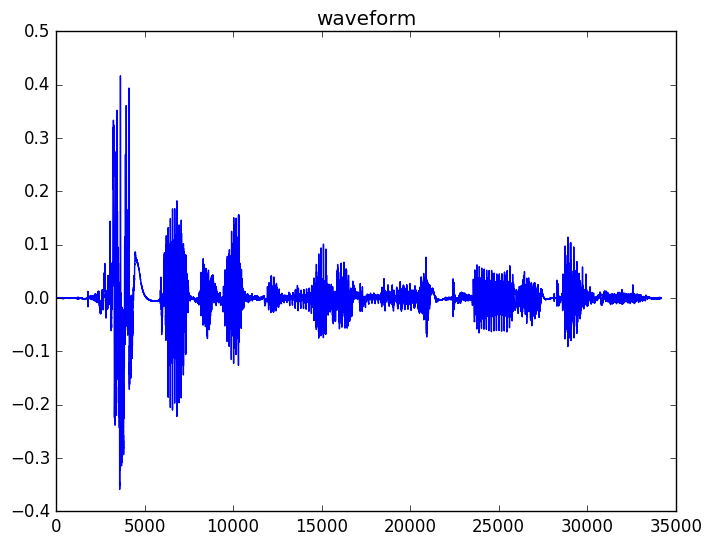
\includegraphics[width=0.45\textwidth]{waveform}
  \hspace{1cm}
  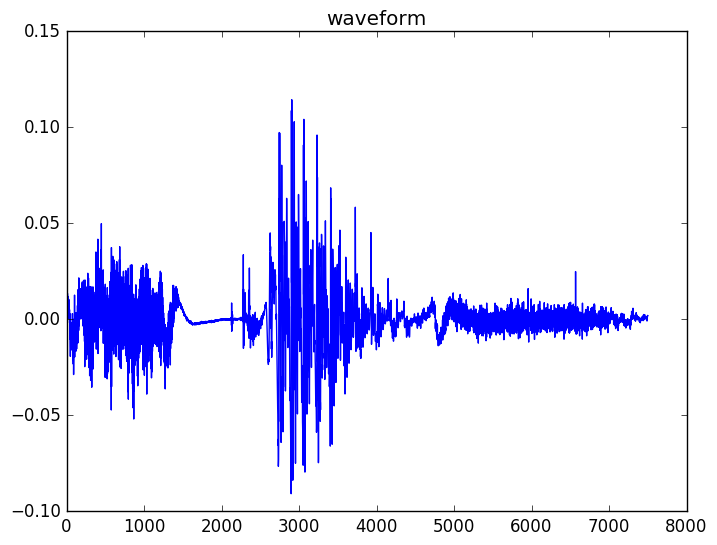
\includegraphics[width=0.45\textwidth]{stuff}
  \hspace{1cm}
  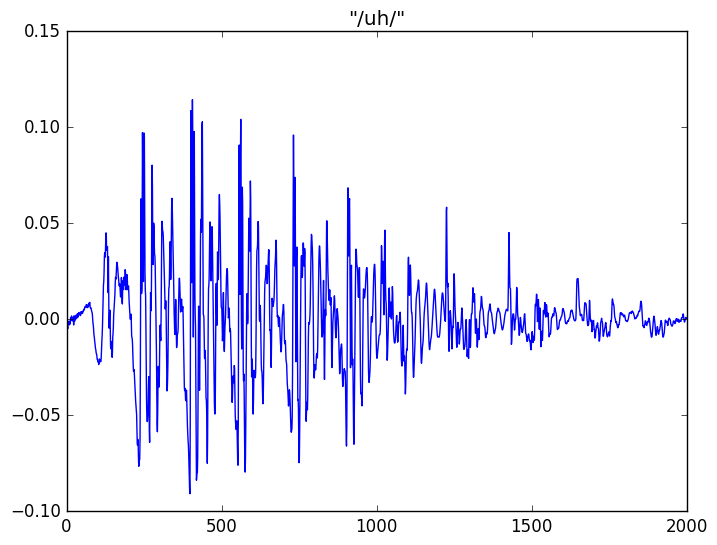
\includegraphics[width=0.45\textwidth]{uh}
  \caption{完整音频波形图与部分波形图}
\label{fig:wavform}
\end{figure}

回忆上一节中讨论的发声音素和不发声音素,我们来瞅一下最后一个单词 "stuff" 的波形图,如图\ref{fig:wavform}(右)。从图上我们看到,这个单词的发音有三个不同的部分,初始不发声语音"st",中间发声语音"uh",终止不发声语音"f"。不发声的语音部分看上去像噪音,具有随机性。而发声部分的语音由于声带的振动而具有周期性。

在拉近一点,我们看看发声的这个元音"/uh/",如图\ref{fig:wavform}(下)可以更明显的看到这个元音的周期性。

从这些波形图中,我们可以看到波形的特征形成有两方面的因素:(1)声带的应激反应(excitation)趋势着空气从声道和嘴巴流出;(2)发出某种特定声音时,声道本身的形状。

举例来说,图\ref{fig:wavform}(右)中"st"和"f"看上去都像噪声,但是他们的形状却不相同,就是因为他们是不一样的声音。而"uh"的声音更具周期性,因为发声的应激反应,其由于发声的时候声道的作用有独特的形状。所以对于同一个说话人来说,不同的元音可能会有着相近的周期,但是波形的整体形状是不一样的,就因为这些波形都是由相同的声带产生的,但是发不同的声音声道是不一样的。

在信号处理中,一般用源滤波器模型(source-filter model)来对这个语音产生的过程进行建模。声源是由通过声道的声带产生的激励信号,我们将其建模成为时变线性滤波器。源滤波器在语音识别中有很多应用,比如语义分析和编码。而且有很多种办法来评估源信号和滤波器的参数,比如很有名的线性预测编码(Linear Predictive Coding,LPC)。

对于语音识别来说,音素分类在很大程度上取决于声道的形状,也就是说取决于源滤波器模型的滤波器部分。激励信号或者原信号大都被忽略或者舍弃了。所以语音识别的特征提取过程一般设计成捕捉话语过程的时变滤波器形状。
% subsection introduction (end)

\subsection{Feature Extraction} % (fold)
\label{sub:feature_extraction}
从波形图中,很明显语音是非平稳信号(non-stationary signal),这就意味着语音信号的统计特性会随着时间变化而变化。所以为了分析语音信号,我们需要将信号分成一个又一个 chunk(也成为窗或者帧),这些chunk短到可以认为它们是平稳信号。这样我们就可以去分析一系列短时的有重叠的语音帧。在语音识别中,我们一般选窗长为 25ms,窗移位 10ms,也就是说一秒钟会被分成100帧。

因为我们是从一个长音频提取的chunk,所以对于每一个chunk的边缘,我们要进行一些处理。一般对每一帧数据加个窗函数,常用的是汉明窗(Hamming Windows),当然也有用其他窗函数的。定义$m$为某一帧的索引,$n$为采样点的索引,$L$是这一帧采样点的个数,$N$是采样中的偏移量。那么从原始信号中提取出来的每一帧计算公式见\ref{eqn:frame-window}。
\begin{align}
\label{eqn:frame-window}
  x_{m}[n]=w[n] x[m N+n], n=0,1, \ldots, L-1
\end{align}
其中$w[n]$是窗函数。

然后我们利用离散傅里叶变换将每一帧的数据转换到频域,如公式\ref{eqn:fft}。所有现代软件中都可以有效的计算快速傅里叶变换。
\begin{align}
\label{eqn:fft}
  X_{m}[k]=\sum_{n=0}^{N-1} x_{m}[n] e^{-j 2 \pi k n N}
\end{align}

傅里叶表征$X_{M} [k]$是一个很复杂的数,因为它包含了每一帧和每一个频率的频谱幅值(绝对幅值)和相位信息。为了提取特征,我们去掉了相位信息,只考虑幅值 $|X_{m}[k]|$。

频谱图描述了对语音信号进行FFT操作得到的log幅值(或者log-power),如图\ref{fig:log-compare}(右)。横轴是帧索引(单位为10ms),纵轴是频率,其范围是0Hz到采样率的一般,也就是对应的Nyquist频率。图中呈现的是"speech recognition is cool stuff"。在频谱图中,黄色和红色区域表示该区域能量高。
% subsection feature_extraction (end)

\subsection{Mel Filtering} % (fold)
\label{sub:mel_filtering}
从频谱图中可以看出高频的高能量区域大致对应着不发声的辅音,低频的高能量区域大致对应着发声的元音。频谱图中,发声区域的水平线(horizonal lines)呈现的是语音的谐波结构(harmonic structure)。

由于发声区域的谐波结构和不发声区域的随机噪声,频谱中存在着变数(variability)。为了移除这些变数,我们对幅度谱(magnitude spectrum)进行频谱光滑操作。受听觉系统处理语音信号的启发,我们对频谱图进行滤波器组操作(filterbank),该滤波器组对频率轴进行了 approximately logarithmic scale。也就是说随着频率的升高,滤波器也会变得更宽间隔更大。最常用于特征提取的filterbank是 {\bf mel filterbank}。一个 mel filterbank 包含40个滤波器,如图\ref{fig:mel-fbank}。每一个滤波器会对不同频率区间的能量谱求平均。
\begin{figure}[htbp]
  \centering
  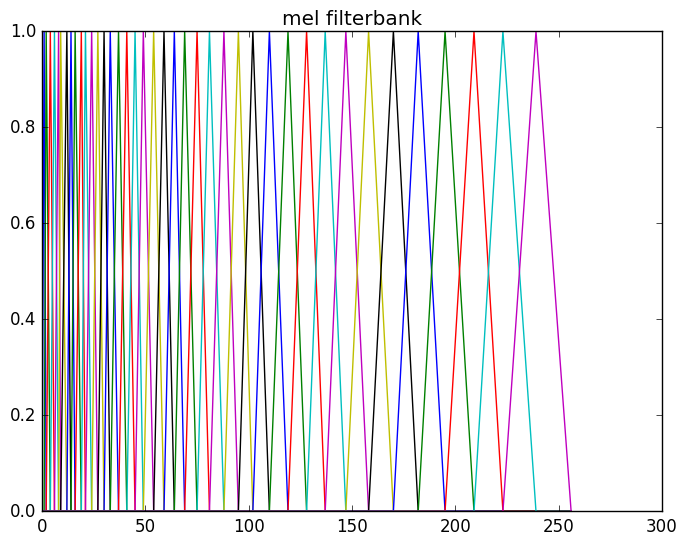
\includegraphics[width=0.45\textwidth]{mel-fbank}
  \caption{mel filterbank \label{fig:mel-fbank}}
\end{figure}

mel filterbank图在左边的滤波器很密集,在右边的滤波器间隔就比较远了。这是符合人耳听觉系统的,因为人耳对低频的信号更加敏感,对高频的信号不太敏感,所以低频的信息是更重要的,那么就需要多一些滤波器,从而提取更多有效特征。

P维的 mel filterbank的系数计算公式如\ref{eqn:mel-fbank}。一个 mel filterbank一般会计算出40个系数,虽然现代系统有的会多一些或者少一些。平滑过多,系数就少一些,反之则反之。
\begin{align}
\label{eqn:mel-fbank}
  X_{\mathrm{mel}}[p]=\sum_{k} M[p, k]\left|X_{m}[k]\right|, \quad p=0,1, \ldots, P-1
\end{align}

% subsection mel_filtering (end)

\subsection{Log Compression} % (fold)
\label{sub:log_compression}
特征提取的最后一步是对经过滤波器组得到的系数进行对数压缩。这个操作有助于压缩信号的动态范围,还能模拟听觉系统对声音的非线性压缩效果。我们把对数压缩后的输出称为 "filterbank" 系数。

将提取的特征以频谱图式的方式呈现出来之后,如图\ref{fig:log-compare}(左),与原始信号频谱图(右)进行比较,我们可以看出沿着频率轴的Fbank系数要平滑得多,这是因为高频噪声和pitch/谐波结构都被移除了。
\begin{figure}[!ht]
  \centering
  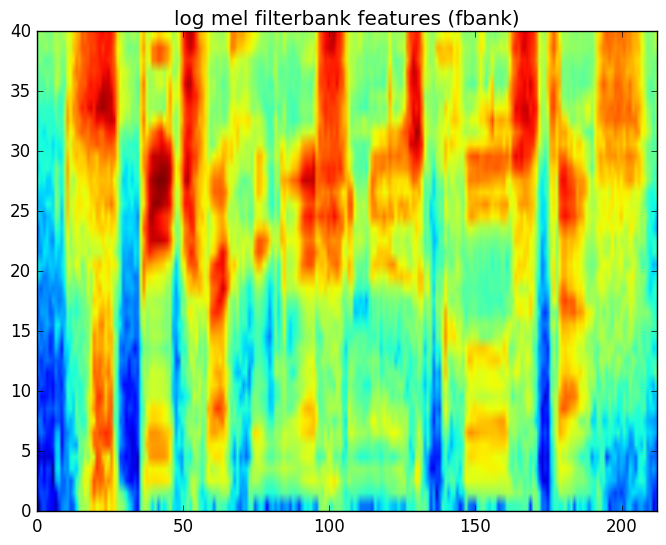
\includegraphics[width=0.45\textwidth]{figure/log-mel-fbank}
  \hspace{1cm}
  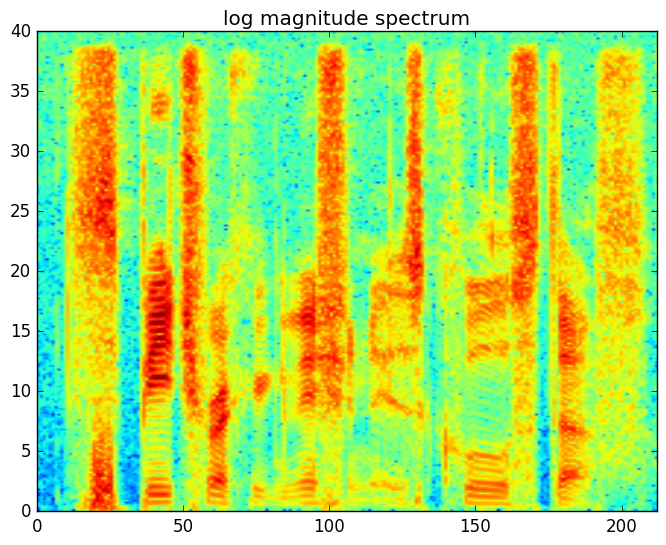
\includegraphics[width=0.45\textwidth]{figure/log-power}
  \caption{提取Fbank特征(左)与原始信号的频谱图(右)}
\label{fig:log-compare}
\end{figure}
% subsection log_compression (end)

除了上面的这些操作,在提取特征的过程中可能还会有一些其他的操作。其中有:
\begin{enumerate}
  \item Dithering(抖动):在原始音频信号中加入一个很小的噪声,为了防止在提取特征的时候出现数学问题,尤其是出现$\log0$;
  \item DC-removal(直流常数移除):在提取特征之前,去除音频中的常数偏置;
  \item Pre-emphasis(预加重):在提取特征之前用一个高通滤波器处理信号,因为发声的语音部分低频能量比不发声的语音部分高频能量要大得多,用一个高通滤波器来抵消下这个问题。实际操作的时候就是用了一个简单地线性滤波器,见公式\ref{eqn:pre-emp},其中$\alpha=0.97$。
    \begin{align}
    \label{eqn:pre-emp}
    y[n]=x[n]-\alpha x[n-1]
    \end{align}
  \item DCT(离散余弦变换):Fbank系数是强相关的,为了减弱这种相关性,将上述步骤提取出来的Fbank特征值再经过DCT。经过DCT之后的特征,一般取前13个,余下的由于所含信息不足舍弃了。DCT公式如\ref{eqn:dct}。
    \begin{align}
    \label{eqn:dct}
    d_t =\frac{\sum_{n=1}^{N}n(c_{t+n}-c_{t-n})}{2\sum_{n=1}^{N}n^2}
    \end{align}
\end{enumerate}}

\subsection{Feature Normalization} % (fold)
\label{sub:feature_normalization}
通信信道可能会对捕获的语音信号引入一些偏差(恒定滤波)。比如说,麦克风的频率响应不平稳,此外,即使相同语音的基础信号,其信号增益的变化也可能导致计算的滤波器组系数的差异。这些信道的影响可以用时域上的卷积进行建模,等价于频域表征的信号进行点乘(elementwise multiplication)。

因此信道的影响可以用恒定滤波来建模(constant filter),如公式\ref{eqn:model-channel}。
\begin{align}
\label{eqn:model-channel}
X_{t, \mathrm{obs}}[k]=H[k] X_{t}[k]
\end{align}
其观测幅度为:
\begin{align}
\label{eqn:ob-mag}
\left|X_{t, \mathrm{obs}}[k]\right|=|H[k]|\left|X_{t}[k]\right|
\end{align}

如果我们对公式\ref{eqn:ob-mag}两边取对数,并计算句子中所有帧的均值,则我们有公式\ref{eqn:log-mean}。
\begin{align}
\begin{split}
\label{eqn:log-mean}
\mu_{\mathrm{obs}}
    &=\frac{1}{T} \sum_{t} \log \left(\left|X_{t, \mathrm{obs}}[k]\right|\right) \\
    &=\frac{1}{T} \sum_{t} \log \left(|H[k]|\left|X_{t}[k]\right|\right) \\
    &=\frac{1}{T} \sum_{t} \log (|H[k]|)+\frac{1}{T} \sum_{t} \log \left(\left|X_{t}[k]\right|\right)\\
\end{split}
\end{align}

假设滤波器在时间轴上是常数,且语音信号的对数幅值均值为0,那么公式\ref{eqn:log-mean}可以简化为\ref{eqn:log-mean-simple}。
\begin{align}
\label{eqn:log-mean-simple}
  \mu_{t t o b s}=\log (|H[k]|)
\end{align}

以上,如果我们计算出句子的对数幅值的均值,并且对句子中的每一帧都减去这个均值,这样我们就可以除去信号中所有的恒定信道效应。

为了简便,我们直接对取了$\log$之后fbank特征进行归一化(normalization)。为了对比一系列操作的结构,图\ref{fig:fbank-normalization}展现了原始信号的频谱图(左)、fbank特征的频谱图(右)和对fbank特征归一化后的频谱图(下)。
\begin{figure}[!ht]
  \centering
  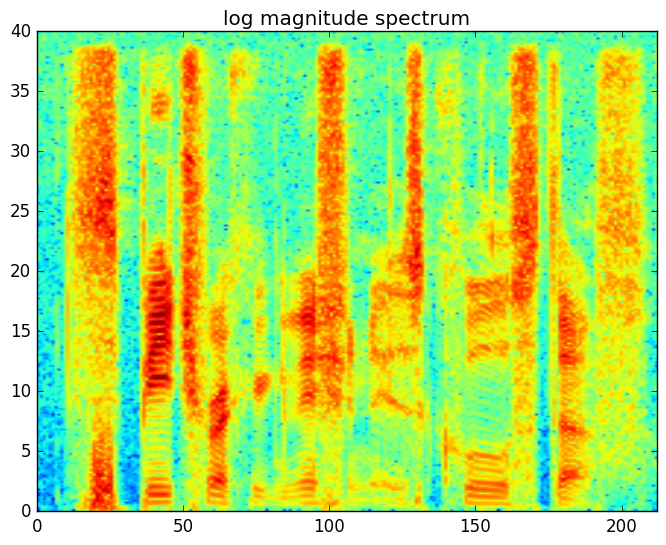
\includegraphics[width=0.40\textwidth]{figure/log-power}
  \hspace{0.5cm}
  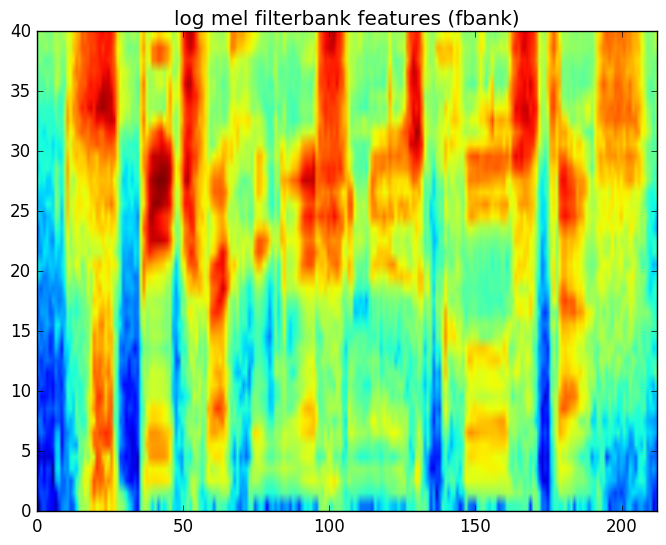
\includegraphics[width=0.40\textwidth]{figure/log-mel-fbank}
  \hspace{0.5cm}
  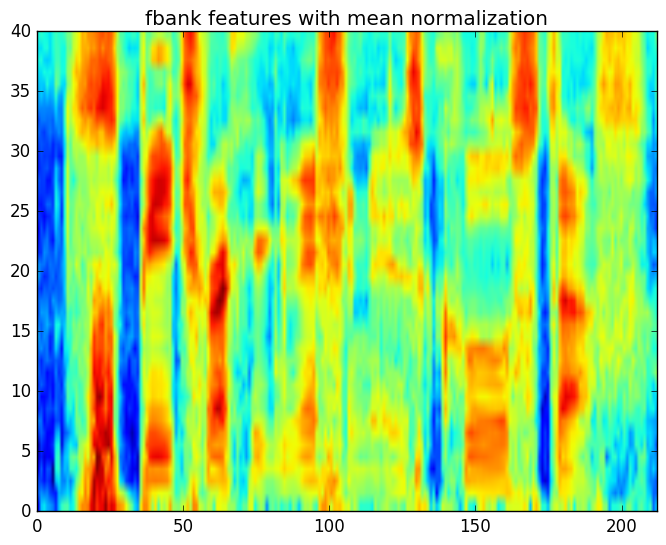
\includegraphics[width=0.40\textwidth]{figure/log-mel-fbank-norm}
  \caption{原始信号的频谱图(左)、提取Fbank特征(右)和归一化后的Fbank特征(下)}
\label{fig:fbank-normalization}
\end{figure}
% subsection feature_normalization (end)
\subsection{Summary}
为了从语音信号中提取语音识别所需的特征,我们希望提取到与声道形状有关的时变频谱信息,其由源滤波器模型中的一个滤波器建模,计算语句中的特征步骤如下:
\begin{enumerate}
  \item 预处理信号,包括预加重和dithering;
  \item 将信号切割成有重叠部分的帧,一般帧长为 25ms,帧移为 10ms;
  \item 对于每一帧:
      \begin{itemize}
        \item 用汉明窗处理信号;
        \item 使用FFT进行傅里叶变换;
        \item 计算频谱的幅值;
        \item 应用 mel filterbank;
        \item 进行对数操作;
      \end{itemize}
  \item 如果需要进行信道补偿,则对每一帧的fbank系数进行均值归一化。
\end{enumerate}}

\subsection{Lab 2: Feature extraction for speech recognition} % (fold)
\label{sub:lab_2}
本模块有一个实验作业,标题为"Feature extraction for speech recognition"。

{\bf Required files:}
\begin{itemize}
  \item \textcolor{blue}{M2\_Wav2Feat\_Single.py}
  \item \textcolor{blue}{M2\_Wav2Feat\_Batch.py}
  \item \textcolor{blue}{speech\_sigproc.py}
  \item \textcolor{blue}{htk\_featio.py}
\end{itemize}}

{\bf Instructions:}

In this lab, you will write the core functions necessary to perform feature extraction on audio waveforms. Your program will convert an audio file to a sequence of log mel frequency filterbank ("FBANK") coefficients.

The basic steps in features extraction are
\begin{enumerate}
  \item Pre-emphasis of the waveform
  \item Dividing the signal into overlapping segments or frames
  \item For each frame of audio:
    \begin{itemize}
      \item Windowing the frame
      \item Computing the magnitude spectrum of the frame
      \item Applying the mel filterbank to the spectrum to create mel filterbank coefficients
      \item Applying a logarithm operation to the mel filterbank coefficient
    \end{itemize}
\end{enumerate}
In the lab, you will be supplied with python file called {\bf speech\_sigproc.py}. This file contains a partially completed python class called {\bf FrontEnd} that performs feature extraction, using methods that perform the steps listed above. The methods for dividing the signal into frames (step 2) will be provided for you, as will the code for generating the coefficients of the mel filterbank that is used in step 3c. You are responsible for filling in the code in all the remaining methods.

There are two top-level python scripts that call this class. The first is called {\bf M2\_Wav2Feat\_Single.py}. This function reads a single pre-specified audio file, computes the features, and writes them to a feature file in HTK format.

In the first part of this lab, you are to complete the missing code in the {\bf FrontEnd} class and then modify {\bf M2\_Wav2Feat\_Single.py} to plot the following items:
\begin{enumerate}
  \item Waveform
  \item Mel frequency filterbank
  \item Log mel filterbank coefficients
\end{enumerate}

You can compare the figures to the figures below. Once the code is verified to be working, the feature extraction program should be used to create feature vector files for the training, development, and test sets. This will be done using {\bf M2\_Wav2Feat\_Batch.py}. This program takes a command line argument {\bf –-set} (or {\bf -s} ) which takes as an argument either {\bf train}, {\bf dev}, or {\bf test}. For example

{\bf \$ python M2\_Wav2Feat\_Batch.py –set train}

This program will use the code you write in the {\bf FrontEnd} class to compute feature extraction for all the files in the LibriSpeech corpus. You need to call this program 3 times, once each for train, dev, and test sets.

When the training set features are computed ({\bf –set train}) the code will also generate the global mean and precision (inverse standard deviation) of the features in the training set. These quantities will be stored in two ASCII files in the {\bf am} direction for use by CNTK during acoustic model training in the next module.

Here are the outputs you should get from plotting:
\begin{figure}[!ht]
  \centering
  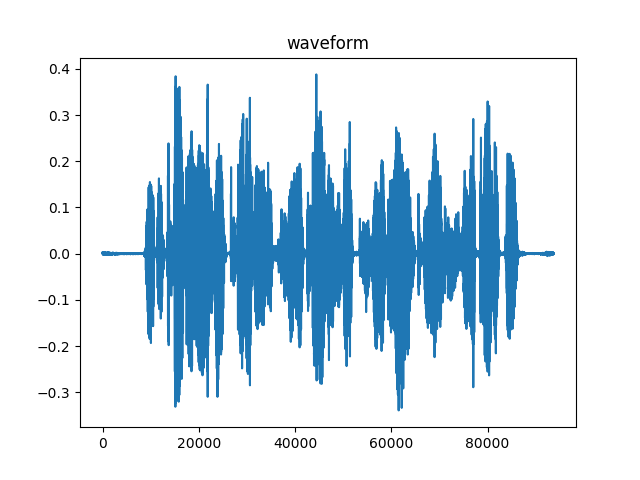
\includegraphics[width=0.30\textwidth]{figure/lab2-1}
  \hspace{0.5cm}
  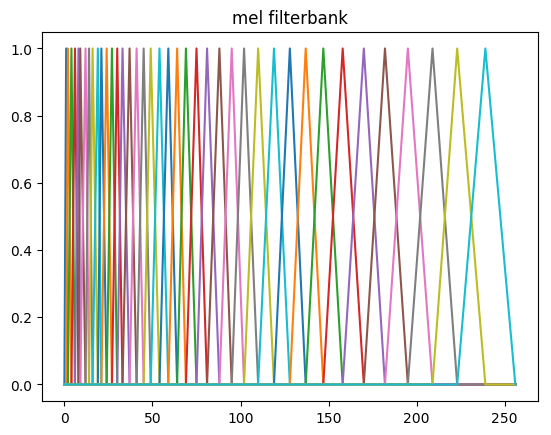
\includegraphics[width=0.30\textwidth]{figure/lab2-2}
  \hspace{0.5cm}
  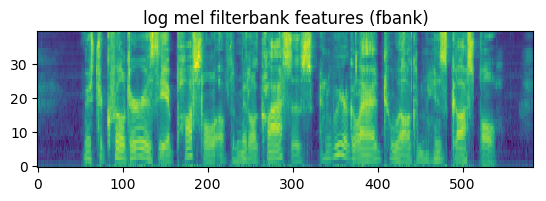
\includegraphics[width=0.30\textwidth]{figure/lab2-3}
  \caption{Lab 2的期望输出}
\label{fig:expect-output}
\end{figure}
% subsection lab_2 (end)

%------------------------------------------------------------------------------
%                                Acoustic Model
%------------------------------------------------------------------------------
\section{Acoustic Modeling}
\subsection{Introduction} 
本节讨论的是语音识别器中的声学模型。声学模型是一个混合模型,通过DNN得到逐帧的预测标签,再通过HMM将这些预测的音素转换成序列预测。HMM常用于对离散时间序列事件的建模。HMM的基本概念可以追溯到数十年前,而且HMM有很多应用。

\subsection{Markov Chains} 
了解一点马尔科夫链(Markov Chains)对学习HMM大有帮助。马尔科夫链是一种对随机过程进行建模的方法。在马尔科夫链中,用一系列状态(states)来对离散时间进行建模。状态之间的运动由随机过程控制。

举例说明,在一个天气预测的应用中,状态为 "{\bf S}unny"、"{\bf P}artly Cloud"、"{\bf C}loudy"、和"{\bf R}aining"。我们考虑某个连续五天的特定天气概率,比如$P(p,p,c,r,s)$,我们可以使用贝叶斯规则将这个联合概率分布打散成一系列条件概率的乘积,如公式\ref{eqn:markov1}。
\begin{align}
\label{eqn:markov1}
  p(X_1, X_2, X_3, X_4, X_5)=p(X_5 | X_4, X_3, X_2, X_1) p(X_4 | X_3, X_2, X_1) p(X_3 | X_2, X_1) p(X_2 | X_1) p(X_1)
\end{align}

假设天气模型满足一阶马尔科夫假设,即满足公式\ref{eqn:first-order}。
\begin{align}
\label{eqn:first-order}
  p(X_i |X_1, ..., X_{i-1})=p(X_i | X_{i-1})
\end{align}

那么连续五天天气的联合概率分布可以简化为公式\ref{eqn:markov2}。
\begin{align}
\label{eqn:markov2}
\begin{split}
  p(X_1, X_2, X_3, X_4, X_5)
      &= p(X_5 | X_4) p(X_4 | X_3) p(X_3 | X_2) p(X_2 | X_1) p(X_1) \\
      &= p(X_1)\prod_{i=2}^{5}p(x_i|x_{i-1})
\end{split}
\end{align}

一个马尔科夫链的核心元素有\textcolor{red}{状态的定义}(此处为天气预测)和\textcolor{red}{转移概率$p(X_i|X_{i-1})$},转移概率描述的是从一个状态移动到另一个状态的概率值(也包括转移到自身状态)。

比如说,天气预报的一个完整的(大体完整的)马尔科夫链可以用图\ref{fig:markov-weather}来表示。
\begin{figure}[htbp]
  \centering
  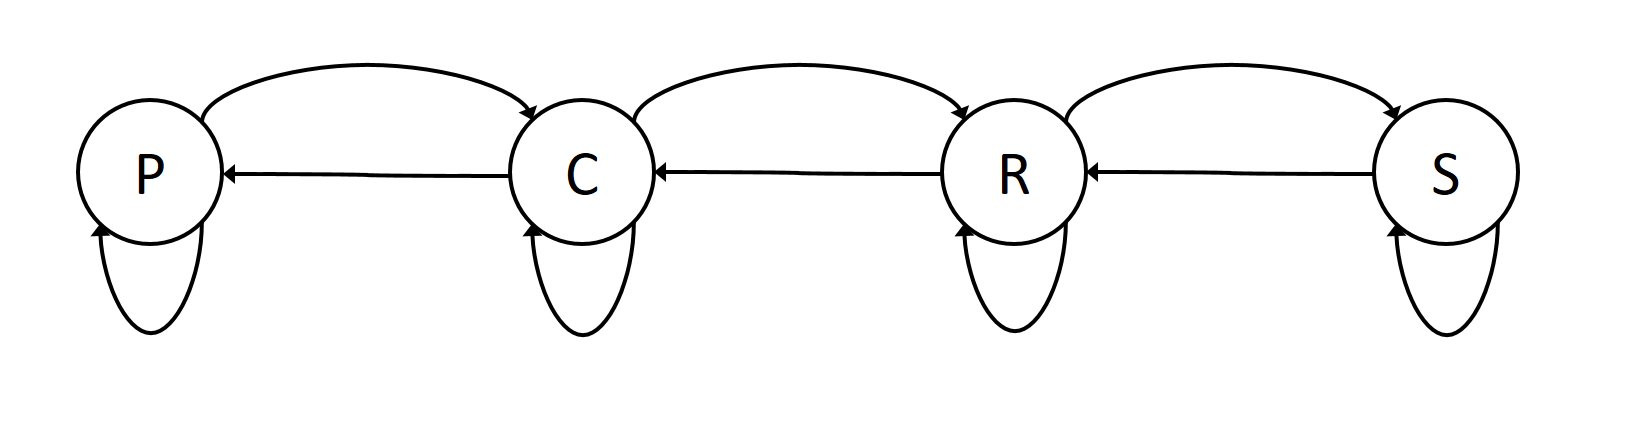
\includegraphics[width=0.45\textwidth]{markov-weather}
  \caption{天气预报模型的马尔科夫链\label{fig:markov-weather}}
\end{figure}

需要注意的是除了上面说的转移概率$p(X_i|X_{i-1})$,我们还需要知道这个序列的第一个元素,即第一天的某种天气的概率值$p(X_1)$。

所以除了状态清单和状态转移概率,我们还需要知道从马尔科夫链每一个状态开始的初始概率值。假设先验概率(每个状态的初始概率值)如公式\ref{eqn:markov-prior}。
\begin{align}
\label{eqn:markov-prior}
\begin{split}
  p(p) &= \pi_{p} \\
  p(c) &= \pi_{c} \\
  p(s) &= \pi_{s} \\
  p(r) &= \pi_{r}
\end{split}
\end{align}

现在我们回到这个例子,公式\ref{eqn:markov-weather-solu}说明了如何求$P(p,p,c,r,s)$。
\begin{align}
\label{eqn:markov-weather-solu}
\begin{split}
  p(p,p,c,r,s) &= p(s|p,p,c,r)p(r|p,p,c)p(c|p,p)p(p|p)p(p) \\
               &= p(s|r) p(r|c) p(c|p) p(p|p) p(p)
\end{split}
\end{align}

\subsection{Problems with Markov Models} 

\subsection{Hidden Markov Models} 

\subsection{Deep Neural Network Acoustic Models} 

\subsection{Training Feedforward Deep Neural Networks} 

\subsection{Using a Sequence based Objective Function} 

\subsection{Lab 3}

%------------------------------------------------------------------------------
%                                Language Modeling
%------------------------------------------------------------------------------
\section{Language Modeling}
\subsection{Introduction} 

\subsection{N gram Models}

\subsection{Language Model Evalution}

\subsection{Operations on Language Models}

\subsection{Advanced LM Topics}

\subsection{Lab 4}

%------------------------------------------------------------------------------
%                                Speech Decoding
%------------------------------------------------------------------------------
\section{Speech Decoding}
\subsection{Overview}

\subsection{Weighted Finite State Transducers}

\subsection{WFSTs and Acceptors}

\subsection{Graph Composition}

\subsection{Lab 5}


%------------------------------------------------------------------------------
%                                Advanced Acoustic Modeling
%------------------------------------------------------------------------------
\section{Advanced Acoustic Modeling}
\subsection{Imporved Objective Functions}

\subsection{Sequential Objective Function}

\subsection{Connectionist Temporal Classsification}

\subsection{Sequence Discriminative Objective Functions}

\subsection{Lab 6}


\section{补充知识点}

\subsection{傅里叶变换}

\subsection{Nyquist定理}